\section{CONSTRUÇÃO DOS ROBÔS}\label{construction}
%% Bruno S. Castro Autor ==================================

Esta secção será destinada à descrição técnica das principais características do robô, referente às suas composições mecânicas e eletrônicas. Além disso, apresentaremos a justificativa das escolhas e seus respectivos benefícios.

\subsection{Estrutura Externa}
%% Bruno S. Castro Autor ==================================

Levando em consideração a facilidade de chegar a estrutura desejada, o custo de produção, trabalho manual envolvido e tempo necessário para construção, decidimos utilizar, após vários testes, impressão 3D com filamento ABS, preenchimento XX\%, altura da camada de XX mm, bico de XX mm e as temperaturas de mesa XX ºC e do bico XX ºC. 

O resultado desta decisão pode ser observado na Figura \ref{fig:visometrica} e superou expectativas, pois obtivemos uma estrutura bem leve (aproximadamente XX gramas), porém suficientemente resistente e modular, com a possibilidade de trabalhar separadamente nos compartimentos mecânico ou eletrônico devido a sua divisão interna, a qual aparenta o robô como um H.

\begin{figure}[htbp]
\centerline{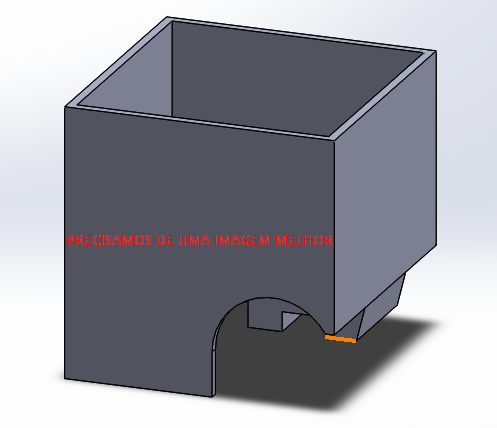
\includegraphics[width=\columnwidth]{capitulos/imagens/robo_visometrica.png}}
\caption{Projeto 3D do robô em vista isométrica}
\label{fig:visometrica}
\end{figure}

Quando o robô precisar de manutenção, podemos ir diretamente ao compartimento mecânico onde temos acesso aos sistemas de movimentação do servo-robô, ou seja, acesso direto aos motores, rodas e conexões entre eles, tal como a fiação elétrica do robô e a bateria de fácil remoção.
Já quando houver a necessidade de acesso ao compartimento eletrônico, teremos contato direto com o sistema de controle responsável pela Rede de Comunicação (disponível na subseção \ref{subsec:rede_com}) do robô. 

\subsection{Sistema de Movimentação}\label{subsec:sist_mov}
%% Bruno S. Castro Autor ==================================

Abaixo descrevemos a composição do nosso Sistema de Movimentação, como pode ser visto na Figura \ref{fig:sist_moviment}, o qual vai ser controlado pela Rede de Comunicação (disponível na subseção \ref{subsec:rede_com}).

\subsubsection{Rodas}
%% Bruno S. Castro Autor ==================================
Quanto ao sistema físico de movimentação do robô, estamos utilizando uma roda composta por um pneu feito com borracha de silicone ultra-resistente de dureza 15 Shore-A acoplado a um cubo de roda feito em Alumínio 6351-T6 especificamente para este pneu. Estes podem ser analisados na Figura \ref{fig:roda}.

\subsubsection{Motores}
%% Bruno S. Castro Autor ==================================
E para completar nosso sistema de movimentação, usamos dois Micro Motores de 6V com caixa de redução para 600 RPM, os quais tem seu eixo fixado as rodas citadas anteriormente. O motor pode ser analisado na Figura \ref{fig:motor}.

\begin{figure}[htbp]
\centering
\begin{subfigure}{0.25\textwidth}
  \centering
  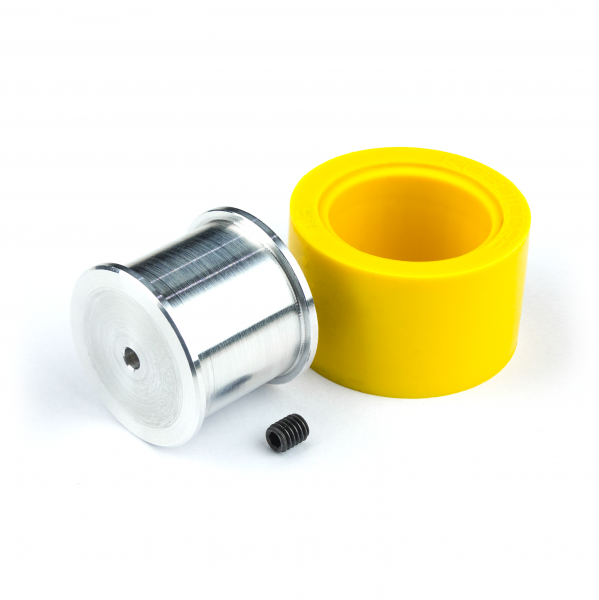
\includegraphics[width=.9\linewidth]{capitulos/imagens/roda_sep.png}
  \caption{Roda utilizada}
  \label{fig:roda}
\end{subfigure}%
\begin{subfigure}{0.25\textwidth}
  \centering
  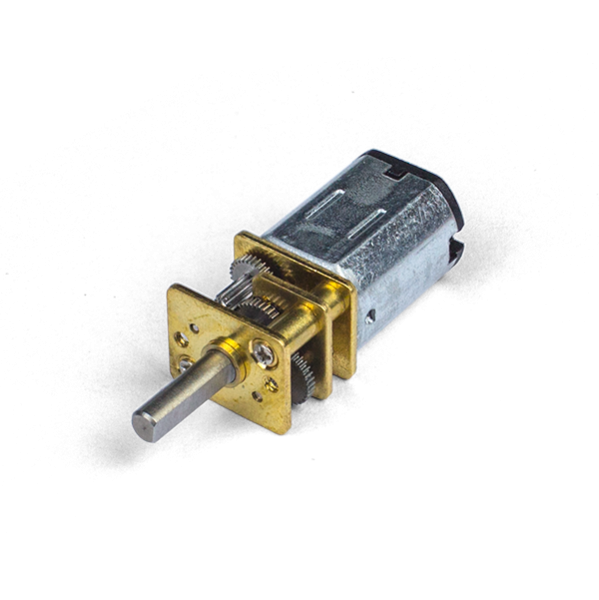
\includegraphics[width=.9\linewidth]{capitulos/imagens/motor.png}
  \caption{Micro Motor utilizado}
  \label{fig:motor}
\end{subfigure}
\caption{Componentes do Sistema de Movimentação}
\label{fig:sist_moviment}
\end{figure}



\subsection{Rede de Comunicação}\label{subsec:rede_com}

\subsubsection{Módulos Receptores}\label{subsec:recept_models}
%% Renan M. Chiesa ==================================

Neste quesito a equipe buscou um sistema de comunicação com uma largura de banda considerável, baixa latência e difícil interferência.
A escolha lógica se afrontou para os módulos de comunicação Xbee\textsuperscript{\textregistered} S2C, os quais se destacam nesses aspectos, porém não possuem um preço adequado para um projeto que não utiliza o envio de dados complexos. 
Desta maneira, buscando não alcançar o limite de projeto orçado, optamos por módulos de comunicação 2.4GHz genéricos mostrados na Figura \ref{fig:modulo_comunication}, estes não chegaram ao desempenho dos módulos Xbee, porém mostraram-se satisfatórios na ocasião. Este modulo possui taxas de transmissão e recepção entre 250kbps e 2Mbps com alcance de até 100 metros, podendo utilizar até 125 canais contendo seis endereços cada, possibilitando assim a conexão com até outras 6 unidades.

\begin{figure}[htbp]
\centerline{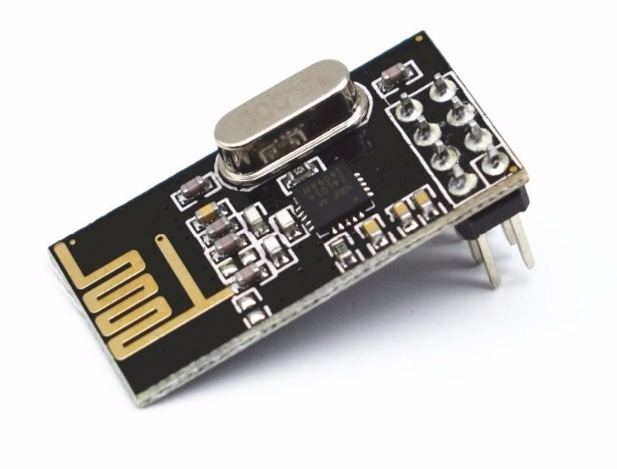
\includegraphics[width=\columnwidth]{capitulos/imagens/modulo_comunication.png}}
\caption{Módulo  NRF24L01}
\label{fig:modulo_comunication}
\end{figure}


\subsubsection{Base de Transmissão}
%% Renan M. Chiesa ==================================

Com o objetivo de estabelecer comunicação entre o sistema de processamento(computador) e cada robô, tivemos a necessidade de construir uma base de envio de dados remotos. Esta base é equipada com uma placa de desenvolvimento Arduino Mega e um módulo de comunicação 2.4 GHz idêntico aos inseridos nos robôs. Está placa foi programada para receber os dados do sistema de processamento por meio do protocolo serial USB, convertendo-os para a estrutura de dados a ser enviada. A comunicação é realizada na faixa de frequência de 2.4GHz(Wi-Fi), está configurada de modo a definir a base como mestre, e cada um dos receptores em modo servo, com estes três recebendo comandos remotos.

As mensagens a serem enviadas possuem formato pré-estabelecido pelo modelo do módulo. Serão enviados na mensagem, dados respectivos ao endereço do receptor do robô com que se deseja a comunicação e os dados necessários ao controle do robô. O envio ocorre várias vezes por segundo possibilitando assim um controle preciso. 


\subsection{Microcontrolador}
%% Alisson Autor ==================================

O microcontrolador escolhido pela equipe para controlar os robôs foi o ATmega328P embarcado na placa Arduino Nano. A preferência por este placa foi em decorrência de suas dimensões diminutas que são de 1,8 cm por 4,8 cm, mostrado na Figura \ref{fig:nano}. Possui todas funções básicas encontradas em placas Arduino porém apresentando algumas configurações diferenciadas, como a alimentação sendo realizada por uma entrada mini-USB e um menor número de portas de entrada e saída. As portas de entrada e saída encontradas nele são suficientes para a operação do robô. 

\begin{figure}[htbp]
\centerline{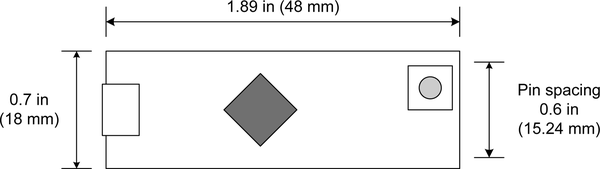
\includegraphics[width=\columnwidth]{capitulos/imagens/arduino_nano.png}}
\caption{Dimensões do Arduino Nano}
\label{fig:nano}
\end{figure}

\section{SISTEMA DE VISÃO}\label{vision}

O propósito da visão computacional é coletar dados do jogo em tempo real que tem como fim descrever o ambiente, e, posteriormente, transmití-los da forma mais compacta possível para o algoritmo responsável pela estratégia.
O processo para a extração dos dados do ambiente é descrito a seguir.
Primeiramente, uma câmera é fixada perpendicularmente ao campo, a aproximadamente 2 metros de altura, faz uma série de captura de imagens individuais, ou \textit{frames}, e os envia para o computador.
Para cada \textit{frame} recebido, utiliza-se um algoritmo para o processamento da imagem com base na biblioteca OpenCV \cite{bradski2008learning}.
Aplicam-se filtros na imagem para obter somente as partes importantes: a bola, as \textit{tags} de cores dos robôs da equipe, e as \textit{tags} da cor que identifica robôs da outra equipe.

Após serem detectadas as etiquetas de cores e a bola, um algoritmo é utilizado para calcular os dados necessários a ser usado como os estados para rede Deep-RL da estratégia, explicada na seção
\ref{strategy}.
Essa rede tem objetivo definir a tomada de decisão dos agentes após receber informações sobre o estado atual do jogo.
Alguns exemplos de dados enviados para a rede são: posição da bola, posição de robôs da equipe e adversários, orientação dos robôs em relação à bola, distância entre bola e gol, distância entre os robôs e a bola, dentre outros. 

O sistema de \textit{tags} de cores a ser utilizado para a detecção dos robôs no campo se dará pelo uso de 2 círculos de 4,5 centímetros de diâmetro cada, posicionados na diagonal.
Uma das etiquetas, localizada mais próxima à parte de trás do robô, possui a cor azul ou amarela, que serve para identificação do time.
A outra etiqueta possui uma cor distinta para cada robô, o que possibilita a diferenciação entre os robôs da equipe.
Através dos círculos, é possível extrair posição e orientação do robô em relação a bola.
A posição de um robô, por exemplo, é dada pelo ponto médio do vetor que liga o centro dos dois círculos.
O sistema de \textit{tags} pode ser visto na Figura $T A L$.

Algumas estratégias são utilizadas para reduzir o custo computacional. Por exemplo, após ter a posição de um robô em determinado \textit{frame}, o próximo processamento de detecção ocorrerá apenas em uma pequena parte da imagem, ao invés de percorrê-la por inteiro, deixando o processo mais otimizado.

\section{ESTRATÉGIA DE JOGO E TÉCNICAS DE CONTROLE}\label{strategy}

Para que os robôs sejam capazes de jogar, é necessário que haja estratégias de jogo, onde seja otimizada a chance de vitória dado o comportamento dos robôs. 
As decisões vão ser feitas através da analise dos dados coletados pela visão computacional, sendo assim definidas como estados da rede. 
A ação tomadas pelos robôs será feita através dos estados em que o ambiente atual do jogo vai estar. 
Esse controle pode ser feito através das técnicas de aprendizado por reforço exploradas em \cite{stone2005reinforcement} e \cite{riedmiller2009reinforcement}. 
%% Mas como os estados e ações no futebol são considerados de alta dimensão 

\subsection{Aprendizado por Reforço Profundo}

O objetivo do aprendizado por reforço profundo (Deep-RL) é controlar um agente em um ambiente na tentativa de maximizar a função de recompensa, mostrado na Figura \ref{fig:rl}.
O algoritmo da rede-Q profunda (DQN) \cite{mnih2013playing} foi capaz de ter um desempenho de nível humano em muitos dos jogos eletrônicos no Atari estimando as ações de um agente.
Contudo, enquanto a DQN pode resolver problemas em um espaço de observação complexo, ele só pode lidar com ações discretas. É possível notar que muitas tarefas, no controle de robótica, tem espaço de ações continuas.
Então a DQN não pode ser aplicada em domínios contínuos e é necessário usar um outro algoritmo capaz de lidar com esse tipo de problema.

\begin{figure}[htbp]
\centerline{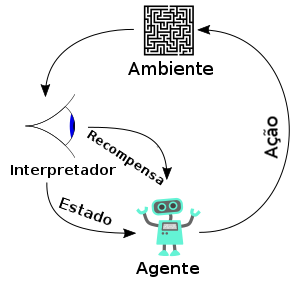
\includegraphics[width=\columnwidth]{capitulos/imagens/reinforcement_learning.png}}
\caption{Ideia principal do funcionamento do agente no Aprendizado por Reforço.}
\label{fig:rl}
\end{figure}

\subsubsection{Soft Actor-Critic (SAC)}

É um algoritmo de Deep-RL baseada na estrutura de entropia máxima para o aprendizado profundo \cite{haarnoja2017reinforcement}.
Nesta estrutura, o rede ator visa maximizar a recompensa esperada enquanto também maximizando a entropia.
Isto é, suceder em uma tarefa enquanto agindo tão aleatória como possível.
Este método é capaz de desempenhar varias atividades em aplicações de domínios contínuos \cite{haarnoja2018soft}.

\subsection{Função de Recompensa para Ataque e Defesa}

Para que a rede Deep-RL seja treinada é necessária uma função de recompensa que permita os agentes fazerem as ações que se é deseja.
Logo, é preciso formular um função de recompensa de ataque e defesa para que assim os agentes consigam jogar futebol.

As principais recompensas definidas para o jogo de futebol são as seguintes:
\begin{multline}
r (s_t, a_t) = r^{gol}_t + p^{gol}_t + c_1(d_{t-1}(b,g) - d_{t}(b,g))\\  + c_2(d_{t-1}(a,b) - d_{t}(a,b))
\end{multline}

Se a rede responsável pelas ações do agente fizer um gol uma recompensa $r^{gol}$ é dada e caso o time leve um gol uma recompensa negativa $p^{gol}$ é dada. Ambas condições representam a maiores recompensas que a rede pode receber por uma ação. 
Caso contrário, a recompensa é baseado na diferença da distância do intervalo de tempo atual com o tempo anterior $(d_{t-1}-d_t)$. Para que o agente se aproxime da bola é usado a distância do agente ao bola $d(a,b)$. Já para que a bola se aproxime do gol adversário é usado a distância da bola ao gol adversário $d(b,g)$.
%% Falta um pouquinho aqui

